\documentclass[11pt, a4paper, oneside]{report}

\usepackage{graphicx}
\usepackage{wrapfig}
\usepackage{lscape}
\usepackage{listings}
\usepackage{xcolor}
\usepackage{rotating}
\usepackage{caption}
\usepackage{subcaption}
\usepackage{amsmath}
\usepackage{upgreek}
\usepackage{gensymb}
\usepackage{csquotes}
\usepackage{pdfpages}
\usepackage{lipsum}
\usepackage{textcomp}
\usepackage{fancyhdr}
\usepackage{setspace}
\usepackage{hyperref}
\usepackage{array}
\usepackage{acronym}
\usepackage[numbers]{natbib}
\usepackage{float}






\usepackage{graphicx}    % Required for inserting images
\usepackage{amsmath}     % For better math formatting
\usepackage{amssymb}     % For additional math symbols
\usepackage{mathrsfs}    % For script letters like \mathscr
\usepackage{amsfonts} % For symbols like \mathbb
\usepackage{amsthm}

\title{SURGE Project}
\author{Anusua Paul}
\date{June *, 2025}

\numberwithin{equation}{section}


\newtheorem{theorem}{Theorem}[chapter]
\newtheorem{corollary}[theorem]{Corollary}
\newtheorem{lemma}[theorem]{Lemma}
\newtheorem{proposition}[theorem]{Proposition}
\newtheorem{remark}[theorem]{Remark}
\newtheorem{note}[theorem]{Note}
\newtheorem{definition}[theorem]{Definition}
\newtheorem{notation}[theorem]{Notation}
\newtheorem{example}[theorem]{Example}


\newcommand{\F}{\mathscr{F}}
\newcommand{\pp}{\mathbb{P}}






\hypersetup{
    colorlinks=true,
    linkcolor=blue,
    urlcolor=blue,
    citecolor=blue
}

\graphicspath{{Figures/}}

% Define custom macros (replace as needed)
\newcommand{\ttitle}{Analysis of the Explicit Exit Time for Brownian Motion in an 
2-Dimensional Lattice Structure}
\newcommand{\authornames}{Anusua Paul}
\newcommand{\supnameA}{Dr. Suprio Bhar}
\newcommand{\supnameB}{Prof. B. Co-supervisor}
\newcommand{\univname}{Indian Institute of Technology Kanpur}
\newcommand{\deptname}{Department of Mathematics and Statistics}
\newcommand{\degreename}{Master of Technology}
\newcommand{\subjectname}{Materials Science}
\newcommand{\keywordnames}{materials, thesis, IITK, engineering}

\title{\ttitle}
\author{\authornames}
\date{\today}

\begin{document}
% -------------------------
% Title Page (Enhanced Layout with Large Logo)
% -------------------------
\begin{titlepage}
\begin{center}
    \vspace*{0.5cm}
    
    % Title
    {\Huge \bfseries \ttitle}\\[0.4cm]
    \rule{0.8\linewidth}{0.8pt} \\[1.2cm]

    % Student Info
    
    {\large \textbf{Anusua Paul}}\\[0.1cm]
    Roll No : \textbf{241080056}\\
    SURGE 2025 Application No : \textbf{2530400}\\[1.5cm]

    % Supervisor
    {\normalsize \textbf{Project Report under the Guidance of}}\\[0.1cm]
    {\normalsize \textbf{Dr. Suprio Bhar}}\\[2cm]

    % Enlarged Logo
    
\includegraphics[width=0.4\linewidth]{pictures/iitk logo.png}\\[1cm]

    % Institute Info
    {\Large \textsc{\deptname}}\\[0.2cm]
    {\Large \textsc{\univname}}\\[2cm]

   

\end{center}
\end{titlepage}


% -------------------------
% Declaration Page (Supervisor)
% -------------------------
\chapter*{Certificate}
\addcontentsline{toc}{chapter}{Certificate}

\noindent
This is to certify that the work presented in the thesis entitled \textbf{\enquote{\ttitle}}, authored by \textbf{\authornames}, has been carried out under my supervision. To the best of my knowledge, this work has not been submitted elsewhere, either in part or in full, for the award of any degree.


\vspace{2cm}

\noindent
\begin{minipage}{0.6\textwidth}
\textbf{\supnameA} \\
Associate Professor\\
\deptname\\
\univname
\end{minipage}


% -------------------------
% Declaration Page (Student)
% -------------------------
\chapter*{Declaration}
\addcontentsline{toc}{chapter}{Declaration}

\noindent
I declare that the work presented in this thesis, titled \textbf{\enquote{\ttitle}}, is the outcome of my independent study project carried out under the supervision of \textbf{\supnameA}.

\medskip

I further affirm that this thesis has not been submitted, either in part or in full, for the award of any degree or diploma at any other academic institution. Due acknowledgment has been made wherever the work of others has been cited or used.

\vspace{2cm}

\noindent
\textbf{\authornames} \\
Roll No. 241080056 \\
\deptname \\
\univname



% -------------------------
% Abstract
% -------------------------
\chapter*{Abstract}
\addcontentsline{toc}{chapter}{Abstract}

We began our study by exploring the relationship between Brownian motion and harmonic functions. This foundational understanding allowed us to delve into the classical Dirichlet problem in electrostatics, which in turn facilitated our investigation into the recurrence and transience properties of Brownian motion in arbitrary dimension.

\noindent As part of this exploration, we also studied key probabilistic tools such as the strong Markov property and Blumenthal’s 0-1 law, particularly focusing on their applications to tail events. These concepts proved instrumental in advancing our theoretical groundwork.

\noindent Subsequently, we transitioned to topics involving the reflection principle and properties of planar Brownian motion. This reading phase concluded with a solid conceptual framework that enabled us to approach the main research article referenced in our study.

\noindent Following the research paper, we sought to understand the derivation of an explicit expression for the exit time of a Brownian motion from an equilateral triangle. The prior theoretical insights were crucial in comprehending this analysis. Building upon that, we attempted to generalize the results to a regular n-gon that spans the two-dimensional plane and aimed to compute the explicit exit time expression for such domains.

% -------------------------
% Acknowledgements
% -------------------------
\chapter*{Acknowledgements}
\addcontentsline{toc}{chapter}{Acknowledgements}

I would like to sincerely thank Dr. Suprio Bhar for his guidance, support, and insightful discussions throughout the course of this project. His mentorship was crucial in shaping my understanding of Brownian motion and related stochastic concepts.
\noindent I also thank IIT Kanpur and the SURGE program for providing this valuable research opportunity. Lastly, I am grateful to my family and peers for their constant encouragement during this project.



% -------------------------
% Table of Contents, List of Figures/Tables
% -------------------------
\tableofcontents

% -------------------------
% Chapters
% -------------------------
\chapter{Harmonic Functions and Dirichlet Problem }
In this section we explore the relation between the Brownian Motion and Harmonic functions. This study will help us to explore the transience and recurrence property of Brownian motion for different dimensions and will provide us the answer to the fundamental Dirichlet problem of electrostatics. 

\noindent Suppose \(U \) is a domain that is a connected open set \(U \subset \mathbb{R}^d\) and \(\partial{U}\) be it's boundary with closure \(\bar{U}\) which is homogeneous and boundary of which is electrically charged. The charge is given by a continuous function \(\varphi : \partial{U} \to \mathbb{R}\). In the Dirichlet problem we want to find the voltage \(u(x)\) at any \(x \in U\). By Kirchoff law \(u\) must be harmonic in \(U\). Now we start our discussion by defining Harmonic functions.

\begin{definition}[{\cite[Definition 3.1]{PeresMortersBook}}]
Suppose \(U \subset \mathbb{R}^d\) is a domain. A function \(u : U \to \mathbb{R}\) is called a \(\boldsymbol{Harmonic\ function}\) on \(U\) if it is twice continuously differentiable and for all \(x \in U\) satisfies the following equality \\
\[
\Delta u(x) = \sum_{i=1}^{d} \frac{\partial^2 u(x)}{\partial x_i^2} = 0
\]
If \(\Delta{u}(x) \geq 0\) then we call it a \(\boldsymbol{subharmonic\ function}\).
\end{definition}
\begin{theorem}[{\cite[Theorem 3.2]{PeresMortersBook}}]
Suppose \(U \subset \mathbb{R}^d\) and \(u : U \to \mathbb{R}^d\) is a function which is measurable and locally bounded then the following statements are equivalent .
\begin{enumerate}
 \item u is harmonic .
 \item for any \(\mathbb{B}(x,r)\subset U\)
 \[
u(x) = \frac{1}{\mathscr{L}(\mathbb{B}(x, r))} \int_{\mathbb{B}(x, r)} u(y) \, dy
\]
where \(\mathscr{L}(\mathbb{B}(x,r))\) is the d dimensional volume of the ball ( for \(d=1\) it is length, for \(d=2\) it is area, for \(d=3\) it is volume and so on ).
 \item for any \(\mathbb{B}(x,r) \subset U\)
\[
u(x) = \frac{1}{\sigma_{x,r}(\partial \mathbb{B}(x, r))} \int_{\partial \mathbb{B}(x, r)} u(y) \, d\sigma_{x,r}(y)
\]
where \(\sigma_{x,r}(\partial \mathbb{B}(x, r))\) is the surface measure of the boundary of the ball (for \(d = 3\), it is the surface area of the 3-dimensional sphere).
\end{enumerate}
Note that this is referred to as mean value property .
\end{theorem}
\begin{remark}[{\cite[Remark 3.3]{PeresMortersBook}}]
Green's identity:
\[
\int_{\partial \mathbb{B}(x, r)} \frac{\partial u}{\partial n}(y) \, d\sigma_{x,r}(y) = \int_{\mathbb{B}(x, r)} \Delta u(y) \, dy 
\]
where \( n(y) \) represents the unit outward normal vector to the boundary \( \partial \mathbb{B}(x, r) \) at the point \( y \).

\end{remark}
\begin{proof}
First we prove \((2) \implies (3)\)\\
Define \(\psi(r) : (0,\infty) \to \mathbb{R}\) such that 
\[
\psi(r) = r^{1 - d} \int_{\partial \mathbb{B}(x, r)} u(y) \, d\sigma_{x, r}(y)
\]
For any \(r >0\)


\[
r^d \, \mathscr{L}(\mathbb{B}(x,1)) \, u(x) = \mathscr{L}(\mathbb{B}(x,r)) \, u(x)
\]

Put \( d = 2 \)

\[
\text{Then } \mathscr{L}(\mathbb{B}(x,1)) = \pi
\]
\[
\mathscr{L}(\mathbb{B}(x,r)) = \pi r^2
\]

The equality holds.

Put \( d = 3 \)

\[
\text{Then } \mathscr{L}(\mathbb{B}(x,1)) = \frac{4}{3} \pi
\]
\[
\mathscr{L}(\mathbb{B}(x,r)) = \frac{4}{3} \pi r^3
\]

So the equality holds.\\
Proceeding this way we can show this for any dimension d .\\

\noindent From (2) we have
\[
\mathscr{L}(\mathbb{B}(x,r))\,U(x) = \int_{\mathbb{B}(x,r)} U(y)\,dy = \int_0^r \psi(s)\,s^{d-1}\,ds
\]

\noindent Note that for \( d \geq 2 \), here \( x \) and \( y \) are \( d \)-dimensional vectors.  
Let us try to prove this for \( d = 2 \).  
Consider the following transformation, \( (y_1, y_2) \Rightarrow (s, \theta) \)

\[
\begin{aligned}
    y_1 &= s \cos \theta \\
    y_2 &= s \sin \theta
\end{aligned}
\quad \quad
\begin{aligned}
    0 \leq s \leq r \\
    0 < \theta \leq 2\pi
\end{aligned}
\]

So we have
\[
\int_{\mathbb{B}(x,r)} U(y)\,dy = \int_{\mathbb{B}((x_1,x_2),r)} U(y_1,y_2)\,dy_1\,dy_2
\]

The Jacobian of the above transformation is \( s \), so

\[
= \int_0^{2\pi} \int_0^r U(s\cos\theta, s\sin\theta)\,s\,ds\,d\theta
\]

Let \( \vec{z} = (s\cos\theta, s\sin\theta) \), and define the surface measure on the boundary \( \partial \mathbb{B}(x,s) \) as \(\sigma_{x,s}(\vec{z}\) and \( d\sigma_{x,s}(\vec{z}) = s\,d\theta \). Then,

\[
= \int_0^r \left( \int_0^{2\pi s} U(\vec{z})\,d\sigma_{x,s}(\vec{z}) \right) ds\\
=\int_0^r \psi(s) s ds
\]
\noindent So the equality holds for \(d = 2\).
Proceeding this way we can show the below equality holds for any \(r > 0 \) and \(d \in \mathbb{N}\)
\[
r^d \, \mathscr{L}(\mathbb{B}(x,1)) \, u(x) = \int_0^r \psi(s)\,s^{d-1}\,ds
\]
Now differentiate both sides of the equality with respect to \( r \):
\[
d\, r^{d-1} \mathscr{L}(\mathbb{B}(x,1))\, u(x) = \psi(r)\, r^{d-1}
\]

Again we know,  
\[
d\, r^{d-1} \mathscr{L}(\mathbb{B}(x,1)) = \sigma_{x,r}(\partial \mathbb{B}(x, r))
\]

Put \( d = 2 \):  
\[
d\, r^{d-1} \mathscr{L}(\mathbb{B}(x,1)) = 2\pi,\quad \sigma_{x,r}(\partial \mathbb{B}(x, r)) = 2\pi
\]
\noindent Thus for \( d = 2 \), the equality holds and it can be shown that the equality will hold for any \( d \).

Then,  
\[
\sigma_{x,r}(\partial \mathbb{B}(x, r))\, u(x) = \psi(r)\, r^{d-1}
\]
and hence,
\[
u(x) = \frac{1}{\sigma_{x,r}(\partial \mathbb{B}(x, r))} \int_{\partial \mathbb{B}(x,r)} u(y)\, d\sigma_{x,r}(y)
\]
where the last equality follows from the definition of $\psi(r)$. This completes the proof of \((2) \implies (3)\).


\noindent Now we prove \( (3) \implies (2) \).\\
From (2) we have  
\[
u(x)\, \sigma_{x,r}(\partial \mathbb{B}(x,r)) = \int_{\partial \mathbb{B}(x,r)} u(y)\, d\sigma_{x,r}(y)
\]

Fix \( s > 0 \).  
Integrating both sides with respect to \(r\) where \(0 \leq r \leq s\), we get 
\[
u(x) \int_0^s \sigma_{x,r}(\partial \mathbb{B}(x,r))\, dr = \int_0^s \left( \int_{\partial \mathbb{B}(x,r)} u(y)\, d\sigma_{x,r}(y) \right) dr
\]

Now from the previous proof 
\[
\int_0^s\left(\int_{\partial \mathbb{B}(x,r)}u(y)\, d\sigma_{x,r}(y)\right)dr = \int_{\mathbb{B}(x,r)} u(y)\, dy
\]

For \( d = 2 \), we have:
\[
\int_0^s\int_{\partial \mathbb{B}(x,r)} u(y)\, d\sigma_{x,r}(y)\, dr = \int_0^s \int_0^{2\pi r} u(y)\, d\sigma_{x,r}(y)\, dr = \int_{\mathbb{B}(x,s)}u(y)\, dy
\]

Thus, it can be shown for any dimension \( d \).\\

Also,
\[
\int_0^s \sigma_{x,r}(\partial \mathbb{B}(x,r))\, dr = \mathscr{L}(\mathbb{B}(x,s))
\]
So the equality of (2) is proved.

\noindent Now we show, (3) \(\implies\) (1). Using convolution we can show that \( u \) is infinitely often differentiable in \( U \). Now suppose \( \Delta u \ne 0 \), so \( \exists \, \mathbb{B}(x, \varepsilon) \subset U \) such that \( \Delta u(x) > 0 \) on the ball or \( \Delta u(x) < 0 \) on the ball then 
using the previous notations.

\[
\psi(r) = d\mathscr{L}(\mathbb{B}(x,1)) \, u(x)
\]
and hence differentiating this w.r.t. \( r \)
\[
0 = \psi'(r) = r^{1-d} \int_{\partial \mathbb{B}(x,r)} \frac{\partial u}{\partial n}(y) \, d\sigma_{x,r}(y)
= r^{1-d} \int_{\mathbb{B}(x,r)} \Delta u(y) \, dy
\]
\noindent which is a contradiction to the fact that 
on the ball \( \mathbb{B}(x,r) \) either \( \Delta u(x) > 0 \) or 
\( \Delta u(x) < 0 \). So \( \Delta u(x) = 0 \), implying the harmonicity.

\noindent Finally we are to show,\(
(1) \Rightarrow (3)
\). 
\noindent  Given \( u \) is harmonic and \( \mathbb{B}(x, r) \subset U \) \\
Then using Green's identity we have,

\[
\psi'(r) = r^{1-d} \int_{\partial \mathbb{B}(x,r)} \frac{\partial u}{\partial n}(y) \, d\sigma_{x,r}(y) = r^{1-d} \int_{\mathbb{B}(x,r)} \Delta u(y) \, dy = 0
\]
\noindent so \( \psi(r) \) is constant in \( r \). \\
As \( u(x) \) is harmonic so it is continuous in the domain thus when \( r > 0 \) is very small \( \Rightarrow \exists \varepsilon >0 \) such that
\[
|u(x) - u(y)| < \varepsilon \quad \text{for any } y \in \mathbb{B}(x,r)
\]
As \(r \to 0\) we can write
\begin{align*}
|\psi(r)| 
&= r^{1-d} \left| \int_{\partial \mathbb{B}(x,r)} [u(y) - u(x) + u(x)] \, d\sigma_{x,r}(y) \right| \notag \\
&\leq r^{1-d} \int_{\partial \mathbb{B}(x,r)} |u(y) - u(x)| \, d\sigma_{x,r}(y) 
+ |u(x)| \int_{\partial \mathbb{B}(x,r)} d\sigma_{x,r}(y) \notag \\
&= r^{1-d} \left( \int_{\partial \mathbb{B}(x,r)} |u(y) - u(x)| \, d\sigma_{x,r}(y) 
+ |u(x)| \, \sigma_{x,r}(\partial \mathbb{B}(x,r)) \right) \notag \\
&\leq r^{1-d} \left( \varepsilon + |u(x)| \right) \, \sigma_{x,r}(\partial \mathbb{B}(x,r)).
\end{align*}
\noindent As \(\varepsilon \to 0\)
\[
\psi(r)= r^{1-d} \sigma_{x,r}(\mathbb{B}(x,r)) u(x)
\]
From which the equality in (3) follows from the definition of \(\psi(r)\).


\end{proof}
\begin{remark}[{\cite[Remark 3.4]{PeresMortersBook}}]
A twice continuously differentiable function \(u : U \to \mathbb{R}\) is called subharmonic if and only if for any \(\mathbb{B}(x,r) \subset \mathbb{R}^d\) the following inequality holds
\[
u(x) \leq \frac{\int_{\mathbb{B}(x,r)} u(y)dy}{\mathscr{L}(\mathbb{B}(x,r))}
.\]
\end{remark}
\noindent Now we discuss a key property of harmonic and subharmonic functions that is maximum principle .
\begin{theorem}\label{maximum}
[{\cite[Theorem 3.5]{PeresMortersBook}}]
\textbf{Maximum Principle :} Suppose \(U \subset \mathbb{R}^d\) is an open connected set and \(u : U \to \mathbb{R}\) is a subharmonic function defined. Then 
\begin{enumerate}
  \item If \(u\) attains maximum in \(U\) then \(u\) is a constant function .
 \item If \(u\) is continuous on \(\bar{U}\) and \(U\) is bounded then
 \[
 max_{x \in \bar{U}} u(x) =  max_{x \in \partial{U}} u(x)
. \]  
\end{enumerate}
\end{theorem}

\begin{proof}
Define \(V =  \{x \in U : u(x)  = M\} \)  where M is the maximum. From the construction it is clear that \(V\) is relatively closed in \(U\). Now consider any such \(x \in V\) . Then for that \(x\) there exist a ball \( \mathbb{B}(x,r) \subset U\) as \(U \) is open. Using mean value theorem for subharmonic function we get \\
\[
M=u(x) \leq \frac{\int_{\mathbb{B}(x,r)} u(y)dy}{\mathscr{L}(\mathbb{B}(x,r))} \leq M
\]
Thus \( \forall\ y \in \mathbb{B}(x,r)\ u(y)=M\). Thus by continuity \(\mathbb{B}(x,r) \subset V\) . So \(V \) is also open. Again previously we had \(V\) is relatively closed in \(U\). Together this two implies that \(U=V\). So \(u\) is constant in \(U\).
\noindent Given that \(u\) is continuous in \(\bar{U}\) and it is closed and bounded . Then using continuity property and the previous statement of this theorem the maximum should be attained on \(\partial{U}\).
\end{proof}
\begin{remark}[{\cite[Remark 3.6]{PeresMortersBook}}]
If \(u\) is harmonic then the above theorem can be made for for \(u\) as well as \(-u\). In that case the maximum will just be replaced by the minimum.
\end{remark}
\begin{corollary}\label{unique}[{\cite[Corollary 3.7]{PeresMortersBook}}]
Suppose \( u_1,u_2 : \mathbb{R}^d \to \mathbb{R}\) harmonic functions on a bounded domain \(U \subset \mathbb{R}^d\) and continuous on it's closure \(\bar{U}\). If \(u_1,u_2\) agrees on \(\partial{U}\) then they are identical .
\end{corollary}
\begin{proof}
By Theorem \ref{maximum} applied to \(u_1 -u_2\) we get 
\[
max_{x\in \bar{U}}{\{u_1(x)-u_2(x)\}} = max_{x\in \partial{U}}{\{u_1(x)-u_2(x)\}} = 0 
\]
Hence \(u_1(x) \leq u_2(x) \forall x \in \bar{U}\) . Applying the same for \(u_2-u_1\) we get the inequality \(u_2(x) \leq u_1(x) \forall x \in \bar{U}\) which  follows the inequality \(u_1(x) = u_2(x) \forall x \in \bar{U}\).
\end{proof}
\noindent Now after discussing all this properties of harmonic functions we proceed towards discussing the relation between harmonic functions and Brownian motion.
\begin{theorem}\label{locally-bounded-harmonic-function}[{\cite[Theorem 3.8]{PeresMortersBook}}]
Suppose \( U \) is a domain, and let \( \{B(t): t > 0\} \) be a Brownian motion started at \( x \in U \). Define the stopping time
\[
\tau = \tau(\partial U) := \inf\{t > 0 : B(t) \in \partial U\}
\]
as the first hitting time of the boundary \( \partial U\). Let \( \varphi: \partial U \to \mathbb{R} \) be a measurable function such that the function \( u: U \to \mathbb{R} \), defined by
\[
u(x) = \mathbb{E}_x \left[ \varphi(B(\tau)) \, \mathbf{1}_{\{\tau < \infty\}} \right], \quad \text{for every } x \in U,
\]
is locally bounded. Then \( u \) is a harmonic function.

\end{theorem}
\begin{remark}[{\cite[Theorem 2.16]{PeresMortersBook}}]
\textbf{Strong Markov Property :} 
For every almost surely finite stopping time \( T \),  
the process  
\[
\{ B(T + t) - B(T) : t > 0 \}
\]  
is a standard Brownian motion independent of \( \mathcal{F}^{+}(T) \).\\
where \( \mathcal{F}^{+}(T) = \bigcap_{s > t} \sigma(B(t) : 0 \leq t \leq s)\).

\end{remark}
\begin{proof}
The proof is followed from the strong markov property and mean value theorem of harmonic functions . For any ball \(\mathbb{B}(x,r) \subset U\) let \(
\tilde{\tau} = \inf\{t > 0 : B(t) \notin \mathbb{B}(x, \delta)\}
\). Then by strong markov property we have ,

\[
u(x) = \mathbb{E}_x \left[ \varphi(B(\tau)) \, \mathbf{1}_{\{\tau < \infty\}} \right]
\]

\[
= \mathbb{E}_x \left[ \mathbb{E}_{B(\tilde{\tau})} \left[ \psi(B(\tau)) \, \mathbf{1}_{\{\tau < \infty\}} \middle| \mathcal{F}^+(\tilde{\tau}) \right] \right]
\]
As after fixing the filtration the starting point of the Brownian motion is shifting at \(B(\tilde{\tau})\) and becoming independent of the filtration by the strong markov property.

\[ u(x)
= \mathbb{E}_x \left[ u(B(\tilde{\tau})) \right]
= \int_{\partial \mathbb{B}(x,\delta)} u(y) \, \nu_{x,\delta}(dy) \quad 
\]
where \(\nu_{x,\delta}\) denotes the uniform distribution over \(\partial{\mathbb{B}(x,r)}\). Given u is locally bounded and we have shown that it also satisfies the mean value property. So u is harmonic .



\end{proof}
\begin{definition}[{\cite[Definition 3.9]{PeresMortersBook}}]
Suppose \(U \subset \mathbb{R}^d \) and \(\partial{U}\) be it's boundary . Suppose \(\varphi : \partial{U} \to \mathbb{R}\) is continuous function on it's boundary. A continuous function \(v : \bar{U} \to \mathbb{R}\) is a solution to this \textbf{Dirichilet\ Problem} with boundary value \(\varphi\) if it is harmonic on \(U\) and \(v(x)=\varphi(x)\) for \(x \in \partial{U}\).
\end{definition}
\begin{remark}
Note that it is not always necessary that there will always exist a solution to a Dirichlet problem. However for some sufficiently nice domain \(U\) the solution exists.
\end{remark}
\begin{definition}
[{\cite[Definition 3.10]{PeresMortersBook}}]
Let \( U \subset \mathbb{R}^d \) be a domain. We say that \( U \) satisfies the \emph{Poincaré cone condition} at a boundary point \( x \in \partial U \) if there exists a cone \( V \) with vertex at \( x \), opening angle \( \alpha > 0 \), and height \( h > 0 \), such that
\[
V \cap \mathbb{B}(x, h) \subset U^c,
\]
where \( \mathbb{B}(x, h) \) denotes the open ball of radius \( h \) centered at \( x \), and \( U^c \) is the complement of \( U \).
\end{definition}
\noindent Let us discuss some property of this type of domains which have solution to the dirichlet problem. Note that for any set \(A \subset \mathbb{R}^d\) the first hitting time of the set \(A\) by the Brownian motion is given by \(\tau(A) = inf\{ t \geq 0 : B(t) \in A\}\).
\begin{lemma}[{\cite[Lemma 3.11]{PeresMortersBook}}]
Let \( 0 < \alpha < 2\pi \), and let \( C_0(\alpha) \subset \mathbb{R}^d \) be a cone with vertex at the origin and opening angle \( \alpha \). Define
\[
a = \sup_{x \in cl \mathbb{B}(0, \frac{1}{2})} \mathbb{P}_x\left( \tau(\partial \mathbb{B}(0,1)) < \tau(C_0(\alpha)) \right),
\]
Then \( a < 1 \). Moreover, for any positive integer \( k \) and any \( h_0 > 0 \), we have
\[
\mathbb{P}_x\left( \tau(\partial \mathbb{B}(z, h_0)) < \tau(C_z(\alpha)) \right) \leq a^k,
\]
for all \( x, z \in \mathbb{R}^d \) satisfying \( |x - z| < 2^{-k} h_0 \), where \( C_z(\alpha) \) denotes the cone with vertex at \( z \) and opening angle \( \alpha \).

\end{lemma}

\begin{theorem}\label{Dirichlet-problem}
[{\cite[Theorem 3.12]{PeresMortersBook}}]
\textbf{Dirichlet Problem :} Suppose \( U \subset \mathbb{R}^d \) is a bounded domain such that every boundary point satisfies the Poincaré cone condition, and suppose \( \varphi \) is a continuous function on \( \partial U \). Let 
\[
\tau(\partial U) = \inf\{ t > 0 : B(t) \in \partial U \}
\]
be an almost surely finite stopping time. Then the function
\[
u(x) = \mathbb{E}_x[\varphi(B(\tau(\partial U)))], \quad \text{for all } x \in \overline{U},
\]
is the unique continuous function harmonic on \( U \) with \( u(x) = \varphi(x) \) for all \( x \in \partial U \).

\end{theorem}
\begin{figure}[htbp]
    \centering
    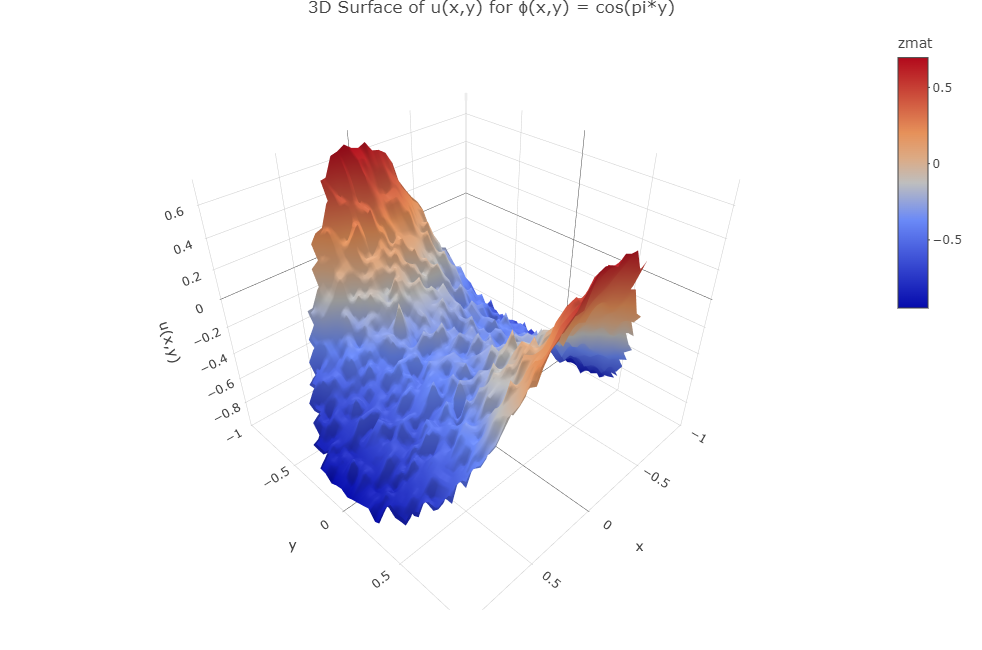
\includegraphics[width=0.9\textwidth]{dirichlet.png}
    \caption{3-d surface of u(x,y) for  $\varphi(x,y)= cos (\pi y)$}
\end{figure}

\begin{proof}
Let us do the proof step by step. First we show that the expectation exists.
Given \(\tau(\partial U)\) is finite almost surely. So \(B(\tau(\partial(U)\) is also finite. As \(\bar{U}\) is bounded and \(\varphi\) is continuous so \(\varphi(B(\tau(\partial U)))\) is also finite almost surely. So the expectation is also finite and exists.
\noindent As finite so bounded and this implies locally bounded then by Theorem \ref{locally-bounded-harmonic-function} \(u\) is a harmonic function.
\noindent Now we are to proof that \(u\) is continuous on \(\bar{U}\). Fix \( z \in \partial U \), then there is a cone \( C_z(\alpha) \)
based at \( z \) with angle \( \alpha > 0 \) with \( C_z(\alpha) \cap \mathbb{B}(z, h') \subset U^c \). By Lemma 3.11, 
for any positive integer \( k \) and \( h' > 0 \), we have
\[
\mathbb{P}_x \left\{ \tau(\partial \mathcal{B}(z, h')) < \tau(C_z(\alpha)) \right\} \leq a^k
\]
for all \( x \) with \( |x - z| < 2^{-k} h' \). Given \( \varepsilon > 0 \), there is a \( 0 < \delta \leq h' \) such that 
\( |\varphi(y) - \varphi(z)| < \varepsilon \) for all \( y \in \partial U \) with \( |y - z| < \delta \). 
For all \( x \in \overline{U} \) with \( |z - x| < 2^{-k} \delta \),
Now \[
|u(x)-u(z)| = | \mathbb{E}_x[\varphi(B(\tau(\partial U)))]-\varphi(z)|
\text{ (As it is given on boundary \(u\) and \(\varphi\) matches )} 
\]
so,
\[
|u(x)-u(z)| \leq \mathbb{E}_x[|\varphi(B(\tau(\partial U)))-\varphi(z)|] 
\]
Now define an event \[A=\left\{ \tau(\partial \mathbb{B}(z, h')) < \tau(C_z(\alpha)) \right\}\]
We can write ,
\[
\mathbb{E}|\varphi(B(\tau(\partial U)))-\varphi(z)|=
\mathbb{E}_x[|\varphi(B(\tau(\partial U)))-\varphi(z)|I_A + |\varphi(B(\tau(\partial U)))-\varphi(z)|I_{A^c}] \leq 
\]
\[
2 \| \varphi \|_{\infty} \, \mathbb{P}_x \left\{ \tau(\partial \mathbb{B}(z, \delta)) < \tau(C_z(\alpha)) \right\} + 
\varepsilon \, \mathbb{P}_x \left\{ \tau(\partial U) < \tau(\partial \mathbb{B}(z, \delta)) \right\} 
\leq 2 \| \varphi \|_{\infty} a^k + \varepsilon.
\]
where \(||\varphi \|_{\infty}\) is the norm supremum .
\[
|\varphi(B(\tau(\partial U)))-\varphi(z)| \leq |\varphi(B(\tau(\partial U)))|+|\varphi(z)| \leq 2||\varphi \|_{\infty}
\]
which implies \(u \) is continuous on \(\bar{U}\). Which follows from Corollary \ref{unique} the uniqueness of \(u\).



\end{proof}
\noindent Note that if poincare cone condition hold at every boundary point of the domain then one can simulate the solution of the Dirichlet problem just by knowing the \(\varphi\) function.
\begin{example}
[{\cite[Example 3.15]{PeresMortersBook}}]    
Consider a solution \( v : \mathbb{B}(0,1) \to \mathbb{R} \) of the Dirichlet problem on the planar disc \( \mathbb{B}(0,1) \), with boundary condition \( \varphi : \partial \mathbb{B}(0,1) \to \mathbb{R} \). Let 
\[
U = \{ x \in \mathbb{R}^2 : 0 < |x| < 1 \}
\]
denote the punctured disc. We claim that the function
\[
u(x) = \mathbb{E}_x \left[ \varphi\left( B(\tau(\partial U)) \right) \right]
\]
does not solve the Dirichlet problem on \( U \) with boundary condition \( \varphi : \partial \mathbb{B}(0,1) \cup \{0\} \to \mathbb{R} \), assuming \( \varphi(0) \neq v(0) \). 

\noindent The reason is that planar Brownian motion almost surely does not hit isolated points. Hence the first hitting time \( \tau \) of the boundary \( \partial U = \partial \mathcal{B}(0,1) \cup \{0\} \) almost surely coincides with the first hitting time of \( \partial \mathcal{B}(0,1) \). Therefore, by Theorem \ref{Dirichlet-problem}
\[
u(0) = \mathbb{E}_0 \left[ \varphi\left( B(\tau) \right) \right] = v(0) \neq \varphi(0).
\]
This demonstrates that \( u \) fails to satisfy the prescribed boundary condition at the origin.
\end{example}
\noindent Now we apply the techniques we developed to prove a classical theorem of harmonic function that is the Liouville's theorem by probabilistic means. This uses the \textbf{Reflection principle} for higher dimensional Brownian motion.
\begin{theorem}
[{\cite[Theorem 3.16]{PeresMortersBook}}]
All bounded harmonic function in \(\mathbb{R}^d\) is constant.
\end{theorem}
\begin{proof}
Let \(u : \mathbb{R}^d \to [-M,M]\) be a harmonic function. Let \(x\) and \(y\) be two points in the domain. Let \(H\) be the hyperplane reflection in which takes point \(x\) to \(y\). Let \(\{B(t) : t \geq 0\}\) be the brownian motion started at \(x\) and let  \(\{\bar{B}(t) : t \geq 0\}\) be the reflected brownian motion at time point \(\tau = inf \{t : B(t) \in H\}\). 
\begin{equation}\label{reflection-principle}
\{B(t) : t \geq \tau(H)\} \overset{d}{=} \{\overline{B}(t) : t \geq \tau(H)\}. 
\end{equation}

Since \( u \) is harmonic, we know that \( \mathbb{E}_x[u(B(t))] = u(x) \). Splitting the expectation based on whether \( t < \tau(H) \) or \( t \geq \tau(H) \), we obtain
\[
u(x) = \mathbb{E}_x\left[u(B(t)) {1}_{\{t < \tau(H)\}} \right] + \mathbb{E}_x\left[u(B(t)) {1}_{\{t \geq \tau(H)\}} \right].
\]
Thus we can write 

\begin{align*}
|u(x)-u(y)| 
&= \Big| \mathbb{E}_x\left[u(B(t)) {1}_{\{t < \tau(H)\}} \right] 
+ \mathbb{E}_x\left[u(B(t)) {1}_{\{t \geq \tau(H)\}}\right] \\
&\quad - \mathbb{E}_y\left[u(\bar{B}(t)) {1}_{\{t < \tau(H)\}} \right] 
- \mathbb{E}_y\left[u(\bar{B}(t)) {1}_{\{t \geq \tau(H)\}} \right] \Big|
\end{align*}
\noindent As from equation (\ref{reflection-principle}) we get that \(\{B(t) : t \geq \tau(H)\}\) started at \(x\) is in distribution same as \(\{\bar{B}(t) : t \geq \tau(H)\}\) starting at \(y\). So we get 
\[
\mathbb{E}_x\left[u(B(t)) {1}_{\{t \geq \tau(H)\}}\right] = \mathbb{E}_y\left[u(\bar{B}(t)) {1}_{\{t \geq \tau(H)\}} \right] 
\]
\begin{align*}
|u(x) - u(y)| 
&= \left| \mathbb{E}\left[u(B(t)) {1}_{\{t < \tau(H)\}}\right] 
- \mathbb{E}\left[u(\bar{B}(t)) {1}_{\{t < \tau(H)\}}\right] \right| \\
&\leq 2M \mathbb{P}\{t < \tau(H)\} \longrightarrow 0 \quad \text{as } t \to \infty.
\end{align*}
Therefore, \( u(x) = u(y) \). Since \( x \) and \( y \) were arbitrary, it follows that \( u \) must be constant.
\end{proof}

\chapter{Recurrence and Transience of Brownian Motion}

Suppose 
\[
B_t(\omega) : (\Omega, \F, \pp) \times [0, \infty) \to (\mathbb{R}^d, \mathbb{B}(\mathbb{R}^d))
\]
is a Brownian motion in dimension \( d \). It is called \textbf{transient} if
\[
\lim_{t \to \infty} |B_t(\omega)| = \infty \quad \text{almost surely},
\]
that is,
\[
\pp\left( \left\{ \omega \in \Omega : \lim_{t \to \infty} |B_t(\omega)| < \infty \right\} \right) = 0.
\]
In particular, for fixed \( \omega \in \Omega \), i.e. for a fixed path, we often write \( B_t(\omega) = B(t) \).
Note that  \(
\left\{ \omega :\lim_{t \to \infty} |B_t(\omega)| = \infty \right\}
\) is a \textit{tail event} (as Brownian motion has independence increament property so this event belongs to tail sigma algebra), and hence by the zero-one law for tail events, it happens either with probability 0 or with probability 1. Thus, for fixed \( d \), the Brownian motion is either transient or recurrent.
\begin{definition}
Define \( \mathscr{G}(t) = \sigma(B(s) : s \geq t) \). The \textbf{tail \(\sigma\)-algebra} of Brownian motion  is defined as
\[
\mathscr{T} = \bigcap_{t \geq 0} \mathscr{G}(t),
\]
and consists of all tail events.
\end{definition}
\begin{theorem}[{\cite[Theorem 2.9]{PeresMortersBook}}]
\textbf{Zero-One Law for Tail Events : } Let \( x \in \mathbb{R}^d \) and let \( A \in \mathscr{T} \) be a tail event. Then,
\[
\mathbb{P}_x(A) \in \{0, 1\}.
\]
\end{theorem}
\noindent In this section, we are interested in determining for which dimensions \( d \) Brownian motion is transient, and for which dimensions it is recurrent. This question is closely related to the exit probabilities of a Brownian motion from an annulus.
Consider the annulus
\[
A = \left\{ y \in \mathbb{R}^d : r < |y| < R \right\}, \quad \text{for } 0 < r < R < \infty.
\]
Suppose a Brownian motion starts at a point \( x \in A \). We are interested in the probability that the motion hits \( \partial \mathbb{B}(0, r) \) before it hits \( \partial \mathbb{B}(0, R) \). 
Now, as \( R \to \infty \), we become interested in the event of exit from this annulus. 
The answer to this exit probability is given in terms of a harmonic function defined on the annulus, and is therefore closely related to the \textbf{Dirichlet Problem}. \\
To find an explicit solution \( u : \overline{A} \to \mathbb{R} \) of the Dirichlet problem on an annulus, we first assume that \( u \) is \textbf{spherically symmetric}, i.e., the value of the function depends only on the norm distance \( |x| \) from the origin and not on the angular position. Since the annulus has a symmetric structure, this is a reasonable assumption.
If \( u \) is spherically symmetric, then there exists a function \( \psi : [r, R] \to \mathbb{R} \) such that \(u(x) = \psi(|x|^2).\) \\
We now compute the derivatives of \( u \) in terms of \( \psi \). Letting \( y = |x|^2 \geq 0 \) , we have:
\[
\partial_{i} u(x) = \frac{d}{dx_i} \psi(|x|^2) = \psi'(|x|^2) \cdot 2x_i,
\]
and
\[
\partial_{ii}^2 u(x) = \frac{d^2}{dx_i^2} \psi(|x|^2) = \psi''(|x|^2) \cdot 4x_i^2 + 2\psi'(|x|^2).
\]
Therefore, the Laplacian of \( u \) is
\[
\Delta u(x) = \sum_{i=1}^d \left( 4x_i^2 \psi''(y) + 2\psi'(y) \right).
\]
Now, using the identity \( \sum_{i=1}^d x_i^2 = |x|^2 = y \), we get
\[
\Delta u(x) = 4y \psi''(y) + 2d \psi'(y).
\]
Setting \( \Delta u = 0 \) for harmonicity, we obtain:
\[
4y \psi''(y) + 2d \psi'(y) = 0.
\]
Dividing through by 2, we get:
\begin{align*}
    2y \, \psi''(y) + d \, \psi'(y) &= 0 \\
    \text{and hence , } \psi''(y) + \frac{d}{2y} \, \psi'(y) &= 0
\end{align*}

Here the integrating factor is given by, 

\[
\text{IF} = \exp\left( \int \frac{d}{2y} \, dy \right) = y^{d/2}
\]

Now multiplying with IF we get:

\[
\psi''(y) \, y^{d/2} + \frac{d}{2} \, y^{\frac{d}{2}-1} \, \psi'(y) = 0
\]

\[
\text{and hence , }\frac{d}{dy} \left( \psi'(y) \, y^{d/2} \right) = 0
\]

\[
\text{so} \quad \psi'(y) \, y^{d/2} = \text{const}
\]

\[
\text{and hence , } \psi'(y) = \text{const} \cdot y^{-d/2}
\]
\noindent Thus, \( \Delta u = 0 \) holds for \( |x| > 0 \) as well.
Hence, the general solution \( u(x) \) is given by :
\begin{equation}\label{all-harmonic}
u(x) = 
\begin{cases}
k_1|x| & \text{if } d = 1, \\
k_2\log |x| & \text{if } d = 2, \\
k_d|x|^{2 - d} & \text{if } d \geq 3.
\end{cases}
\end{equation}
where \(k_d \) are constants. Note that for \(d \leq 2\) u(x) is increasing in x and for \(d \geq 3\) onwards it is decreasing in x.\\
Write \( u(r) \) for the value of \( u(x) \) for all \( x \in \partial \mathbb{B}(0, r) \). As \( u(\cdot) \) is spherically symmetric and only depends on the norm distance of \( x \), this is a reasonable notation. Define the stopping times
\[
T_r = \tau(\partial \mathbb{B}(0, r)) = \inf \{ t > 0 : |B(t)| = r \} \quad \text{for } r > 0,
\]
and \( T = T_r \wedge T_R \) denotes  the first exit time from the annulus \( A \). Here, assume that \( T \) is finite almost surely, that is,
\[
\mathbb{P}\left( \left\{ \omega \in \Omega : T(\omega) = \infty \right\} \right) = 0.
\]
From equation \eqref{all-harmonic}, \( u(x) \) is continuous on the annulus, and since every boundary point satisfies the Poincaré cone condition, by Dirichlet Problem , we have
\[
u(x) = \mathbb{E}_x \left[ u(B(T)) \right] = u(r) \, \mathbb{P}_x(T_r < T_R) + u(R)\left(1 - \mathbb{P}_x(T_r < T_R)\right).
\]
From this we can solve for the exit probability
\[
\mathbb{P}_x(T_r < T_R) = \frac{u(R) - u(x)}{u(R) - u(r)},
\]
and this gives the explicit solution to the exit problem.
\begin{theorem}\label{exit-annulus}
[{\cite[Theorem 3.18]{PeresMortersBook}}]
Let \( \{B(t) : t \geq 0\} \) is a Brownian motion in dimension \( d \geq 1 \) started at \( x \in A := \{y \in \mathbb{R}^d : r \leq |y| \leq R \} \), inside an annulus \( A \) with radii \( 0 < r < R < \infty \). Then,
\begin{equation}
\mathbb{P}_x(T_r < T_R) =
\begin{cases}
\displaystyle \frac{R - |x|}{R - r} & \text{if } d = 1, \\[10pt]
\displaystyle \frac{\log R - \log |x|}{\log R - \log r} & \text{if } d = 2, \\[10pt]
\displaystyle \frac{R^{2 - d} - |x|^{2 - d}}{R^{2 - d} - r^{2 - d}} & \text{if } d \geq 3.
\end{cases}
\end{equation}

\end{theorem}


\begin{proof}
The proof directly follows from equation (\ref{all-harmonic}).
\end{proof}
\noindent Letting \( R \uparrow \infty \) in Theorem \ref{exit-annulus} leads to the following corollary.

\begin{corollary}[{\cite[Corollary 3.19]{PeresMortersBook}}]
For any \( x \notin \mathbb{B}(0, r) \), we have
\[
\mathbb{P}_x(T_r < \infty) =
\begin{cases}
1 & \text{if } d \leq 2, \\[10pt]
\displaystyle \left( \frac{r}{|x|} \right)^{d - 2} & \text{if } d \geq 3.
\end{cases}
\]
\end{corollary}
\begin{definition}
Suppose 
\[
X_t(\omega) : (\Omega, \mathscr{F}, \mathbb{\mu}) \times [0, \infty) \to (\mathbb{R}^d, \mathscr{B}(\mathbb{R}^d))
\] is a Markov process . For fixed \(\omega \in \Omega\) write \(X_t(\omega) = X(t)\) .
\begin{itemize}
    \item \textbf{Point recurrent} : if for every \( x \in \mathbb{R}^d \), almost surely, there exists a (random) sequence \( t_n \uparrow \infty \) such that \( X(t_n) = x \) for all \( n \in \mathbb{N} \).
    
    \item \textbf{Neighbourhood recurrent} : if for every \( x \in \mathbb{R}^d \) and \( \varepsilon > 0 \), almost surely, there exists a (random) sequence \( t_n \uparrow \infty \) such that \( X(t_n) \in B(x, \varepsilon) \) for all \( n \in \mathbb{N} \).
    
    \item \textbf{Transient} : if \( |X(t)| \to \infty \) almost surely as \( t \to \infty \).
\end{itemize}
\end{definition}
\begin{theorem}[{\cite[Theorem 3.20]{PeresMortersBook}}]
Brownian motion is
\begin{itemize}
    \item \textbf{point recurrent} in dimension \( d = 1 \),
    \item \textbf{neighbourhood recurrent} but not point recurrent, in dimension \( d = 2 \),
    \item \textbf{transient} in dimension \( d \geq 3 \).
\end{itemize}
\end{theorem}
\begin{remark}[{\cite[Remark 3.21]{PeresMortersBook}}]
\textit{Neighbourhood recurrence}, in particular, implies that the path of a planar Brownian motion (running for an infinite amount of time) is dense in the plane. It means that for any \(x \in R^2\) and for any \( \epsilon > 0\) the Brownian motion will enter in \(B(x,\epsilon)\) infinitely often almost surely.
\end{remark}
\begin{lemma}
\textbf{Paley-Zygmund Inequality : } [{\cite[Lemma 3.23]{PeresMortersBook}}]
For any nonnegative random variable \( X \) with \( \mathbb{E}[X^2] < \infty \),
\[
\mathbb{P}(X > 0) \geq \frac{(\mathbb{E}[X])^2}{\mathbb{E}[X^2]}.
\]
\end{lemma}
\begin{proof}
The Cauchy–Schwarz inequality gives
\[
\mathbb{E}[X] = \mathbb{E}[X \cdot \mathbf{1}_{\{X > 0\}}] \leq \left(\mathbb{E}[X^2]\right)^{1/2} \left(\mathbb{P}(X > 0)\right)^{1/2},
\]
and the required inequality follows immediately by squaring both sides:
\[
\mathbb{P}(X > 0) \geq \frac{(\mathbb{E}[X])^2}{\mathbb{E}[X^2]}.
\]
\end{proof}
\begin{lemma}[{\cite[Lemma 3.24]{PeresMortersBook}}]
Suppose \( E_1, E_2, \ldots \) are events such that
\[
\sum_{n=1}^\infty \mathbb{P}(E_n) = \infty
\quad \text{and} \quad
\liminf_{k \to \infty} \frac{\sum_{m=1}^k \sum_{n=1}^k \mathbb{P}(E_n \cap E_m)}{\left( \sum_{n=1}^k \mathbb{P}(E_n) \right)^2} < \infty.
\]
Then, with positive probability, infinitely many of the events take place, that is,
\[
\mathbb{P} \left( \limsup_{n \to \infty} E_n \right) > 0.
\]
\end{lemma}
\chapter{The Reflection Principle and Path Area }
\section{The Reflection Principle}
Now we will discuss one of the most important application of Strong Markov Property that is the Reflection Principle.
\begin{theorem}[{\cite[Theorem 2.19]{PeresMortersBook}}]
\textbf{(Reflection principle).} If \(T\) is a stopping time and \(\{B(t) : t > 0\}\) is a standard Brownian motion, then the process \(\{B^*(t) : t > 0\}\), called \emph{Brownian motion reflected at \(T\)}, and defined by
\[
B^*(t) = B(t)\mathbf{1}_{\{t \leq T\}} + \big(2B(T) - B(t)\big)\mathbf{1}_{\{t > T\}},
\]
is also a standard Brownian motion.
\end{theorem}
\begin{figure}[htbp]
    \centering
    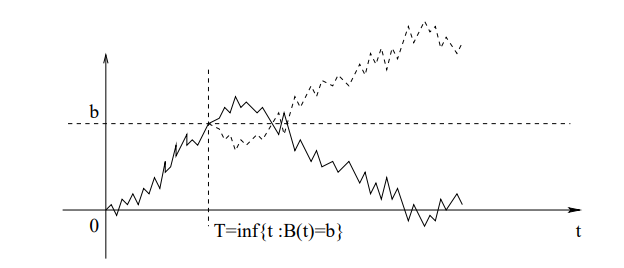
\includegraphics[width=0.9\textwidth]{Screenshot 2025-07-08 162659.png}
    \caption{Reflected Brownian Motion}
\end{figure}

\begin{proof}
Without loss of generality we assume that \(T\) is a finite stopping time. Then by strong markov property 
\[
\{B(T+t)-B(T) : t \geq 0\} \overset{d}{=} \{-B(T+t)+B(T) : t \geq 0\} 
\]
and is independent of the Brownian motion \(\{B(t) : 0 \leq t \leq T\}\). We can write the previous statement as 
\[
\{B(t')-B(T) : t' \geq T\} \overset{d}{=} \{-B(t')+B(T) : t' \geq T\} 
\]
Now on the both side glueing with the independent one Brownian motion we get 
\[
B(t)_{1_{\{t \leq T\}}}+\{B(t)-B(T) \}_{1_{\{t > T\}}}\overset{d}{=} B(t)_{1_{\{t \leq T\}}}+\{-B(t)+B(T) \}_{1_{\{t > T\}}} 
\]
and as for any fixed $\omega \in \Omega$ $B(T)$ is fixed then,
\[B(t)\overset{d}{=}
B(t)_{1_{\{t \leq T\}}}+B(t)_{1_{\{t > T\}}}\overset{d}{=} B(t)_{1_{\{t \leq T\}}}+\{2B(T)-B(t) \}_{1_{\{t > T\}}} 
\]
for any $\omega \in \Omega$ this holds. Here \(B(t)\) is standard Brownian motion and this proves the theorem.

\end{proof}
\begin{theorem}\label{lbm}[{\cite[Theorem 2.8]{PeresMortersBook}}]
Suppose \(\{B(t) : t \geq 0\}\) is a linear Brownian motion started at 0. Define \(\tau=inf\{t \geq 0 : B(t) > 0\}\) and \(\sigma=inf\{t \geq 0 : B(t) = 0\}\) then 
\[
P_0[\tau =0]=P_0[\sigma =0]=1
\]
\end{theorem}
\begin{remark}[{\cite[Remark 2.20]{PeresMortersBook}}]
Define for a standard Brownian motion 
\[
\tau=inf\{t \geq 0 : B(t)= max_{\{0 \leq s \leq 1\}}B(s)\}
\]
and \(\{B^*(t): t \geq 0\}\) be the reflection at time point \(\tau\). Then \(\tau\) is not a stopping time. Note that \(\tau < 1\) so we can add \(t > 0\) which is very small such that \(B(t+\tau)-B(\tau)\) is negative in a small neighbourhood just right of 0 which contradicts Theorem \ref{lbm}. So it is not a stopping time. Also the reflection at this time point is not a Brownian motion.
\end{remark}
\begin{theorem}\label{maximum-theorem}[{\cite[Theorem 2.21]{PeresMortersBook}}]
For a linear Brownian motion define \(M(t)=max_{0 \leq s \leq t}B(s)\). Then if \(a > 0\) 
\[
P_0[M(t)>a]=2P_0[B(t) > a]=P_0[|B(t)|>a].
\]
\end{theorem}
\begin{proof}
Define the stopping time \(T=inf\{t > 0 : B(t)=a\}\) and the reflected Brownian motion at \(T\) as \{\(B^*(t) : t \geq 0\}\). Then
\[
[M(t)>a]=[B(t)>a]\cup [M(t)>a,B(t) \leq a]
\]
Now this two events are mutually disjoint. 
\noindent Again
\[
[M(t)>a,B(t) \leq a] = [M(t)>a,B^*(t) \geq a]=[B(t) \geq a]
\]
which follows from the fact that the reflected Brownian motion is same in distribution as $B(t)$. Then we can write  
\[
P_0[M(t)>a]=P_0[B(t)>a]+P_0[M(t)>a,B(t) \leq a]= 2P_0[B(t)>a]=P_0[|B(t)|>a]
\]
As $B(t)$ and $-B(t)$ has the same distribution.
\end{proof}
\begin{lemma}\label{normal}[{\cite[Lemma 12.9]{PeresMortersBook}}]
Suppose \(X\) is standard normally distributed then for all \(x>0\)
\[
P[X>x] \leq \frac{1}{x} \frac{e^{-x^2/2}}{\sqrt{2\pi}}
\]
\end{lemma}
\begin{remark}[{\cite[Remark 2.22]{PeresMortersBook}}]
Using Lemma \ref{normal} and Theorem \ref{maximum-theorem} we can conclude for any \(a>0\)
\[
P[M(t)>a] \leq \frac{\sqrt{2t}}{a \sqrt{\pi}} {e^{-a^2/2t}}
\]
\section{The area of Planar Brownian motion}
Suppose \(\{B(t) : t\geq 0\}\) is a planar Brownian motion. We denote the lebesgue measure on \(\mathbb{R}^d\) by \(\mathcal{L}_d\) and whenever well defined \(f * g\) denotes the convolution [{\cite[Definition 14.20]{MR4201399}}] of the functions \(f\) and \(g\) as
\[
f*g(x)=\int f(y) g(x-y)dy
\]
for a set \(A \subset \mathbb{R}^d\) and \(x \in \mathbb{R}^d\) then \(A+x=\{a+x : a \in A\}\) is also a measurable space whenever \(A\) is a measurable.
\end{remark}
\begin{lemma}[{\cite[Lemma 2.23]{PeresMortersBook}}]
If \( A_1, A_2 \subset \mathbb{R}^2 \) are Borel sets with positive area, then
\[
\mathcal{L}_2\left( \left\{ x \in \mathbb{R}^2 : \mathcal{L}_2\left( A_1 \cap (A_2 + x) \right) > 0 \right\} \right) > 0,
\]
where \( \mathcal{L}_2 \) denotes the 2-dimensional Lebesgue measure.
\end{lemma}
\begin{proof}
Assume first \(A_1,A_2\) are bounded then the convolution is defined by 
\[
1_{A_1}*1_{-A_2}(x) = \int 1_{A_1}(y)1_{-A_2}(x-y)=\int 1_{A_1}(y)1_{A_2+x}(y)dy= \mathcal{L}_2(A_1 \cap (A_2+x))
\]
Again the area for the set of convolution is given by 
\begin{align*}
\int_{\mathbb{R}^2} \mathbf{1}_{A_1} * \mathbf{1}_{-A_2}(x) \, dx 
&= \int_{\mathbb{R}^2} \int_{\mathbb{R}^2} \mathbf{1}_{A_1}(w) \mathbf{1}_{A_2}(w - x) \, dw \, dx \\
&= \int_{\mathbb{R}^2} \mathbf{1}_{A_1}(w) \left( \int_{\mathbb{R}^2} \mathbf{1}_{A_2}(w - x) \, dx \right) dw \\
&= \mathcal{L}_2(A_1) \cdot \mathcal{L}_2(A_2) > 0
\end{align*}
Thus the convolution is positive on a set of positive area proving the lemma.

\end{proof}
\begin{theorem}\label{levy}[{\cite[Theorem 2.24]{PeresMortersBook}}]
For dimension equals to 2, by L\'evy (1940), almost surely,
\[
\mathcal{L}_2(B[0,1]) = 0.
\]
\end{theorem}
\begin{proof}
Define \(X =\mathcal{L}(B[0,1])\) the area of $B[0,1]$.
Now the question is whether $\mathbb{E}(X)$ exists or not. Note that $X$ is an rv which is always positive. Define $\{W(t) : t \geq 0\}$ an one dimensioanl Brownian motion. Then we can claim 
\begin{align*}
\mathbb{P}(X > a) 
&\leq 2\, \mathbb{P} \left( \max_{t \in [0,1]} |W(t)| > \sqrt{a}/2 \right) \\
& \leq 4\, \mathbb{P} \left( W(1) > \sqrt{a}/2 \right) \\
&\leq 4\, e^{-a/8}
\end{align*}
which implies that $\mathbb{E}(X) < \infty$.
Now $B(3t)$ and $\sqrt{3}B(t)$ has the same distribution and we have 
\[
\mathcal{L}_2(B[0,3]) \leq \sum_{j=0}^{2} \mathcal{L}_2(B[j, j+1])
\]
with equality if and only if for 
\(0 \leq i < j \leq 2\) we have 
\[
\mathcal{L}_2(B[i, i+1] \cap B[j, j+1]) = 0.
\]
Again when \(j = 0,1,2\), we have 
\[
\mathbb{E}\mathcal{L}_2(B[j, j+1]) = \mathbb{E}[X]
\quad \text{and} \quad
3\mathbb{E}[X] = \mathbb{E}\mathcal{L}_2(B[0,3]) \leq \sum_{j=0}^{2} \mathbb{E}\mathcal{L}_2(B[j, j+1]) = 3\mathbb{E}[X].
\]

\noindent
whence, almost surely, the intersection of any two of the \(B[j, j+1]\) has measure zero. In particular, 
\[
\mathcal{L}_2(B[0,1] \cap B[2,3]) = 0
\]
almost surely.
Now we can use the Markov property to define two Brownian motions, $\{B_1(t) : t \in [0,1]\}$ by \(B_1(t) = B(t)\), and 
$\{B_2(t) : t \in [0,1]\}$ by 
$
B_2(t) = B(t+2) - B(2) + B(1).
$
The random variable \(Y := B(2) - B(1)\) is independent of both Brownian motions. For \(x \in \mathbb{R}^2\), let \(R(x)\) denote the area of the set \(B_1[0,1] \cap (x + B_2[0,1])\), and note that \(\{ R(x) : x \in \mathbb{R}^2 \}\) is independent of \(Y\). Then
\[
\mathbb{E}\mathcal{L}_2(B[0,1] \cap B[2,3]) = \mathbb{E}[R(Y)] = (2\pi)^{-1} \int_{\mathbb{R}^2} \mathbb{E}[R(x)] e^{-|x|^2/2} \, dx,
\]
where we are averaging with respect to the Gaussian distribution of \(B(2) - B(1)\). Thus, for \(\mathcal{L}_2\)-almost all \(x\), we have \(R(x) = 0\) almost surely and hence, by Fubini’s theorem [{\cite[pp. 105 - 112]{MR1810041}}],
\[
\mathcal{L}_2\{ x \in \mathbb{R}^2 : R(x) > 0 \} = 0, \quad \text{almost surely.}
\]
which follows that $\mathcal{L}_2(B[0,1]) = 0$ almost surely. This completes the proof.



\end{proof}
\begin{corollary}[{\cite[Corollary 2.26]{PeresMortersBook}}]
For any points \(x, y \in \mathbb{R}^2\), we have
\[
\mathbb{P}_x\{ y \in B(0, 1] \} = 0
\]

\end{corollary}
The proof of this follows from \ref{levy}.

\chapter{Brownian Escape from Equilateral Triangle}\label{sec4}

\section{Motivation} In this chapter we are mainly interested about getting a closed form of the expected exit time of a standard Brownian motion from an equilateral triangle.
\begin{figure}[htbp]
    \centering
    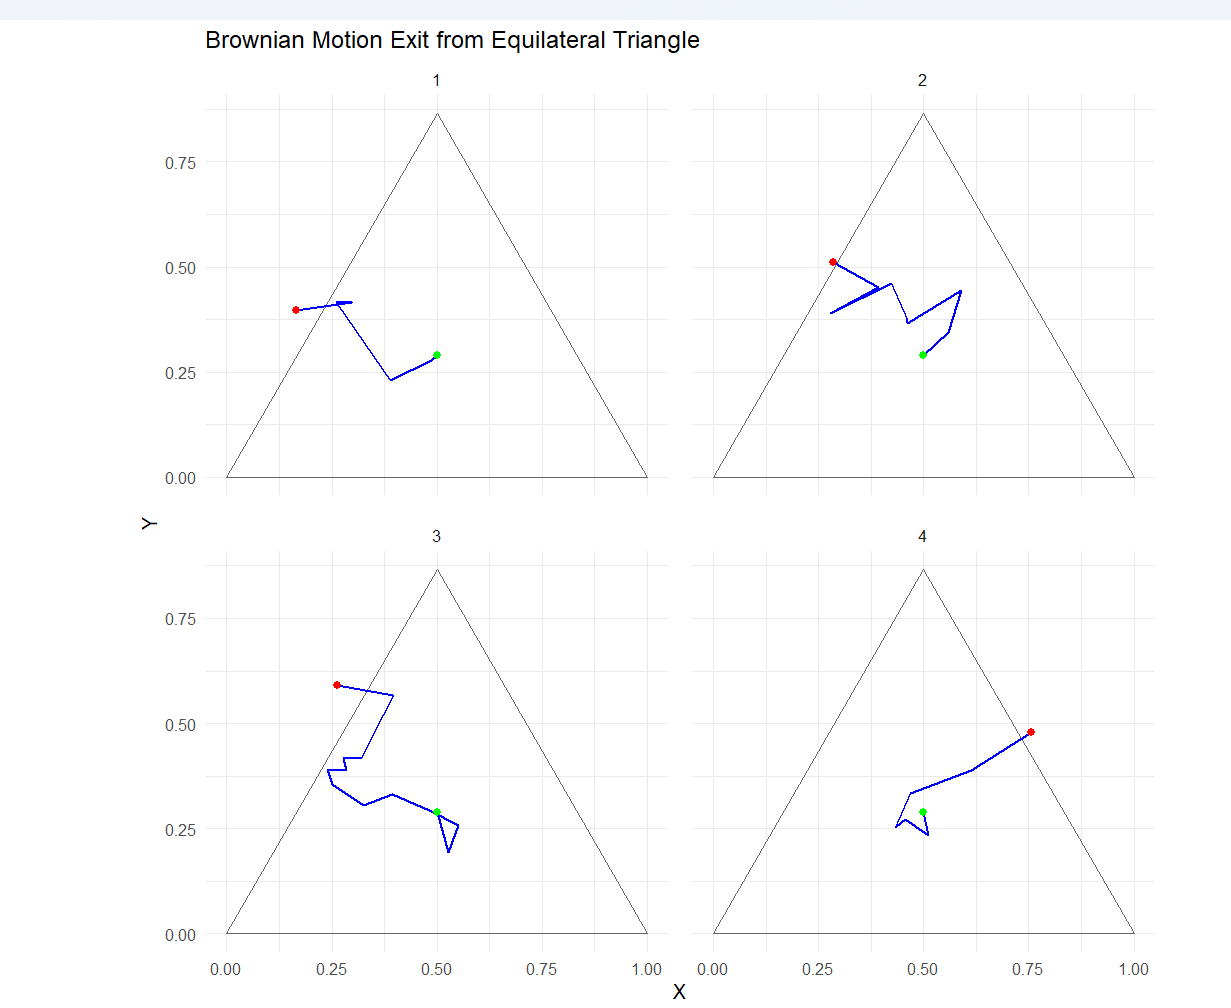
\includegraphics[width=0.5\textwidth]{Screenshot 2025-07-05 141656.png}
    \caption{Exit of Brownian Motion from an Equilateral Triangle}
    \label{fig:Exit_BM_Square}
\end{figure}
In order to do this we firstly construct a Peter, Paul, Mary game which resembles the random walk on triangular lattice covering a 2-d plane. The expected exit time from a triangle located on this triangle lattice is same as the time to ruin of this game. Firstly it is enough to consider here those equilateral triangle with integer side length.
Then we show that this random walk converges in distribution to a standard Brownian motion.
After this we check whether the expected exit time of this random walk also converges to the expected exit time of the Brownian motion from $\Delta_S$ where $S$ is a fixed real number.
Then we scale the random walk down to unit length triangular lattice to compare with the Peter, Paul, Mary game. Thus by comparing with the expected ruin time of the game we get our final expression.


\section{Peter, Paul, Mary game:} There are six possible ways in which we can select a pair from this three people. After selecting the pair we toss a coin to choose who among this pair wins. The person who wins get one rupee from the player who looses among the pair. The other one who is not in the pair does not gain or loose anything.
\section{The lattice and the Laplace equation: }Let $S$ be a positive integer. Consider an equilateral triangle of side length $S$ which is placed on the lattice such that the vertices of $\Delta_S$ are the vertices of the lattice.
Suppose $(\alpha,\beta)$ is the cartesian co ordinate of a vertex of the lattice inside $\Delta_S$ and $(0,0),(S,0),(S/2,\sqrt{3}S/2)$ are the three verteces of $\Delta_S$ then we introduce a new co ordinate system with three co ordinates $(a,b,c)$ where $a,b,c$ corresponds to $(2/\sqrt{3})\beta, \alpha - (1/\sqrt{3}) \beta, S - \alpha - (1/\sqrt{3}) \beta$ respectively. Suppose $h(a,b,c)$ is expected time to ruin of Peter, Paul, Marry problem with begining fortunes as rupees $a,b,c$ respectively. The difference equation which is required to solve is given by,\cite{research}
\begin{align*}
h(a, b, c) =\; &1 + \frac{1}{6} \big( 
    h(a - 1, b + 1, c) + 
    h(a + 1, b - 1, c) + \\
    &\quad\;\; h(a, b - 1, c + 1) + 
    h(a, b + 1, c - 1) + \\
    &\quad\;\; h(a - 1, b, c + 1) + 
    h(a + 1, b, c - 1)
\big)
\end{align*}
with boundary condition 
\[
h(a, b, c) = 0 \quad \text{whenever} \quad \min\{a, b, c\} = 0
\]
Now this difference equation along with this boundary condition has the unique solution.\cite{research}
\[
h(a, b, c) = \frac{3abc}{a + b + c}
\]
\section{Convergence of expected exit time : }
Suppose \(S\) is a positive real number. Now we want to get an explicit expression for the exit time of a 2-D Brownian motion from the equillateral triangle of length \(S\). To do this first we construct a sequence of approximating random walk converging to a standard Brownian motion. Here we use the gambling problem of the previous section. Then we shoe that the expected exit time of the the random walk will also converge to the expected exit time of the limiting distribution.

\noindent Define \(T=inf\{t \geq 0 : X_t \notin \triangle_S\}\) the exit time of the process \(X\) from the triangle of side length \(S\). Let \(\xi_i\) be a sequence of iid random variables taking values $(\cos(k\pi/3), \sin(k\pi/3))$ for \(k=1,2,..5,6\) taking equal probability for each \(k\). It may be thought as a single step on the triangular lattice with side length \(S\). Fix $(\alpha,\beta) \in \mathbb{R}^2$. Define
\begin{equation}
X^n_t=Y^n_{nt} = (\alpha, \beta) + \frac{\sqrt{2}}{\sqrt{n}} \left( \sum_{i=1}^{[nt]} \xi_i + (nt - [ nt])\xi_{[nt] + 1} \right)
\end{equation}
where \( [ \cdot ] \) denotes the integer part.
\begin{proposition}\label{process-convergence}\cite[Proposition 2]{research}
The sequence of processes \( \{X^n_t, \ t \geq 0\} \) converges in law to a standard Brownian motion starting at \( (\alpha, \beta) \).
\end{proposition}


\begin{remark}\label{Donsker}\cite{PeresMortersBook}
\textbf{Donsker's invarience principle}: Let \(\{X_n\}_{n \in \mathbb{N}}\) be a sequence of iid rvs. WLG assume that they are normalized. Define 
\[
S_n = \sum_{k=1}^{n} X_k
\]

\[
S(t) = S_{[ t ]} + (t - [t]) \left( S_{[t ] + 1} - S_{[t]} \right)
\]

Then,
\[
S_n^*(t) = \frac{S(nt)}{\sqrt{n}} = \frac{1}{\sqrt{n}} \left[ \sum_{k=1}^{[[nt]} X_k + (nt - [ nt ]) X_{[ nt ] + 1} \right]
\] 
on the space \(\mathcal{C}[0,\infty)\) of continuous function with metricinduced by norm supremum. The seq $\{S^{*}_n(t): n \geq 1\}$ converges in distribution to a standard Brownian motion starting at origin.
\end{remark}
\begin{remark}\label{multivariate-clt}\cite[Theorem 3.10.7]{MR3930614}
\textbf{Multivariate CLT}: Let \( X_1, X_2, \ldots \) be i.i.d. random vectors with \( \mathbb{E}[X_n] = \mu \), and finite covariances  
\[
\Gamma_{ij} = \mathbb{E}\big[(X_{n,i} - \mu_i)(X_{n,j} - \mu_j)\big].
\]
If \( S_n = X_1 + \cdots + X_n \), then
\[
\frac{S_n - n\mu}{\sqrt{n}} \xrightarrow{d} \chi,
\]
where \( \chi \) has a multivariate normal distribution with mean 0 and covariance matrix \( \Gamma \), i.e.,
\[
\mathbb{E} \left[ \exp(i\theta \cdot \chi) \right] = \exp\left( -\frac{1}{2} \sum_i \sum_j \theta_i \theta_j \Gamma_{ij} \right).
\]
\end{remark}
\begin{proof}
Write \(\xi_i=(\xi_{1i},\xi_{2i})\) where \(\xi_{1i}=cos\ k\pi/3\) and \(\xi_{2i}=sin\ k\pi/3\). Note that \(E(\xi_{1i})=E(\xi_{2i})=0\) and \(V(\xi_{1i})=V(\xi_{2i})=\frac{1}{2}\) and \(E(\xi_{1i} \xi_{2i})=0\). Though the components are not independent they are uncorrelated. Also write 
\[
X^n_{1t}=Y^n_{1nt} = \alpha + \frac{\sqrt{2}}{\sqrt{n}} \left( \sum_{i=1}^{[nt]} \xi_{1i} + (nt - [ nt])\xi_{1[nt] + 1} \right)
\] 
and,
\[
X^n_{2t}=Y^n_{2nt} = \alpha + \frac{\sqrt{2}}{\sqrt{n}} \left( \sum_{i=1}^{[nt]} \xi_{2i} + (nt - [ nt])\xi_{2[nt] + 1} \right)
\]
Then by \ref{Donsker} we have \(X^n_{1t}\) and \(X^n_{2t}\) in distribution converges to a standard Brownian motion starting at respectively \(\alpha\) and \(\beta\). Then using \ref{multivariate-clt} \(X^n_t\) converges in distribution to a 2-D standard Brownian motion started at \((\alpha,\beta)\). Also the tightness of the sequence is followed from the same property for it's scalar components proving the proposition.
\end{proof}
\begin{proposition}\label{exit-time-convergence}\cite[Proposition 3]{research}
The following convergence in law holds:  
\[
T(X^n, \triangle_S) \xrightarrow{d} T(B, \triangle_S).
\]
\end{proposition}
\begin{proof}
Define
\begin{align*}
    \Delta &= \text{open triangle of edge } S \\
    \partial \Delta &= \text{boundary} \\
    \overline{\Delta} &= \text{closure} \\
    T^n &= T(X^n, \Delta) = \text{exit time of the process } X^n \text{ from } \Delta \\
    T &= T(B, \Delta) = \text{exit time of the sbm. } B \text{ from } \Delta
\end{align*}

Note that $B$ is starting at $(\alpha, \beta) \in \Delta$.

Enough to show,
\[
P[T^n > t] \longrightarrow P[T > t] \quad \forall t > 0 \quad \text{as } n \to \infty.
\]

Define \(\mathcal{C} = C([0, \infty), \mathbb{R}^2)\)

\begin{align*}
    X^n &\colon (\Omega, \mathcal{F},P) \times [0, \infty) \longrightarrow (\mathbb{R}^2, \mathcal{B}(\mathbb{R}^2), P^n) \\
    B &\colon (\Omega, \mathcal{F},P) \times [0, \infty) \longrightarrow (\mathbb{R}^2, \mathcal{B}(\mathbb{R}^2), P_B)
\end{align*}

Now,
\[
P[T^n > t] = P^{n} (A)
\]
where
\[
A = \left\{ x \in \mathcal{C} \colon x(0) = (\alpha, \beta) \text{ and } x(s) \in \Delta \ \forall s \le t \right\}
\]

Silly:
\[
P[T > t] = P_B(A)
\]

We can write:
\[
A = \bigcup_{k=1}^\infty \bigcap_{m=1}^\infty \left\{ x \in \mathcal{C} \colon x(0) = (\alpha, \beta) \text{ and } x(s) \in \Delta_{-\frac{1}{k}}\text{ for all } s \in D_m \right\}
\]

Where:
\begin{align*}
    \Delta_{-\frac{1}{k}} &= \Delta - V_{\frac{1}{k}}(\partial \Delta) \\
    V_{\frac{1}{k}}(\partial \Delta) &= \text{$\frac{1}{k}$-th neighbourhood of } \partial \Delta \\
    D_m &= \left\{ \frac{k}{2^m} \colon k \in \mathbb{Z} \right\}
\end{align*}
By the proposition \ref{process-convergence}
\[
P^n(E) \to P_B(E) \quad \text{for all Borel sets } E
\]
with $P_B(\partial E) = 0$ for planar Brownian motion.
By Lévy's theorem, we have $P_B(\partial E) = 0$.
So now it is enough to show 
\[
P_B(\partial A) = 0
\]
then \(P^n(A) \to P_B(A) \) follows from the proposition \ref{process-convergence}
Note that $\mathcal{C}$ is a complete separable metric space under metric
\[
d(x,y) = \sum_{k=1}^{\infty} \frac{1}{2^k} {\|x - y\|_k}
\]
$\| \cdot \|_s$ is sup norm over the compact set $[0, s]$
First we establish that $A$ is an open set in $\mathcal{C}$.
Take any $x \in A$, and $k_0$ is such that 
\[
x(s) \in \triangle_{-\frac{1}{k_0}} \quad \forall s \le t, \text{ $s$ is dyadic}
\]

Set $k = \lfloor t \rfloor + 1$ and $\varepsilon = \frac{1}{2^{k+1}k_0}$

\[
d(x, y) < \varepsilon
\]

\[
\Rightarrow \|y - x\|_t \le \|y - x\|_k < 2^k \varepsilon = \frac{1}{2k_0}
\]

\[
\Rightarrow y(s) \in \triangle_{- \frac{1}{2k_0}} \quad \forall s \le t \quad \text{dyadic}
\]

\[
\therefore \quad y \in A
\]
Closure of \( A \) is
\[
\bar{A} = \left\{ x \in \mathcal{C} : x(0) = (\alpha, \beta) \text{ and } x(s) \in \bar{\Delta} \quad \forall\, s \leq t \right\}
\]

and its boundary is
\[
\partial A = \bar{A} - A 
= \left\{ x \in \mathcal{C} : x(0) = (\alpha, \beta),\, x(s) \in \bar{\Delta} \quad \forall\, s \leq t, \text{ and } x(s') \in \partial \Delta \text{ for some } s' \leq t \right\}
\]

\begin{align*}
\bar{A} - A &= \bar{A} \cap A^c \\
&= \left\{ x \in \mathcal{C} : x(0) = (\alpha, \beta),\, x(s) \in \bar{\Delta} \quad \forall\, s \leq t \right\} \\
&\quad \cap 
\left\{ x \in \mathcal{C} : x(0) = (\alpha, \beta),\, x(s') \notin \Delta \text{ for some } s' \leq t \right\} \\
&= \left\{ x \in \mathcal{C} : x(0) = (\alpha, \beta),\, x(s) \in \bar{\Delta} \quad \forall\, s \leq t,\, 
x(s') \in \partial \Delta \text{ for some } s' \leq t \right\}
\end{align*}
We now decompose \( \partial \Delta \) as the disjoint union of its three edge segments \( r_1, r_2, r_3 \), we obtain
\[
P_B(\partial A) \leq \sum_{i=1}^3 P_B \left( x \in \mathcal{C} : x(0) = (\alpha, \beta),\, x(s) \in \bar{\Delta} \quad \forall\, s \leq t, \text{ and } x(s') \in r_i \text{ for some } s' \leq t \right)
\]
Define the closed half plane \( H_{r_i} \) determined by \( r_i\) containing \( \bar{\triangle_S} \).  
Then we have  
\begin{align*}
&\left\{ x \in \mathcal{C} : x(0) = (\alpha, \beta), \, x(s) \in \bar{\triangle} \quad \forall s \leq t, \, 
\text{and } x(s') \in r_i \text{ for some } s' \leq t \right\} \\
&\subseteq \left\{ x \in \varepsilon : x(0) = (\alpha, \beta) \in H_{r_i} - r_i,\, 
x(s) \in H_{r_i} \quad \forall s \leq t, \, 
\text{and } x(s') \in r_i \text{ for some } s' \leq t \right\}
\end{align*}
Hence it is enough to show  
\[
\left\{ x \in \mathcal{C}: x(0) = (\alpha, \beta) \in H_{r} - r, x(s) \in H_r \forall s \leq t \text{ and }, x(s') \in r\text{ for some } s' \leq t \right\}
\]
This have measure 0.
Now we know that Brownian motion has rotational invarience property. 
By that we can assume \(r\) in the form \( y = m \) and Brownian motion started at \( (0,0) \). Now if we denote 
\[
x(s) = (x^1(s), x^2(s))
\]
Then our required probability is\[
P_B \left[ x \in \mathcal{C},\ x(0) = (0,0),\ x^2(s) \leq m \ \forall s \leq t \text{ and } x^2(s') = m \text{ for some } s' \leq t\right]
\]

Now by continuity of the Brownian motion and Lévy's theorem this probability is equals to 0. This proves the proposition.
\end{proof}
\begin{lemma}\cite[Lemma 4]{research}
The sequence \( \{T(X^n, \triangle_S)\}_{n \in \mathbb{N}} \) is uniformly integrable.
\end{lemma}
\begin{definition}
\textbf{Uniform integrability}:  
A non-empty family \( \mathcal{X} \subseteq L^0 \)  
of random variables is said to be \emph{uniformly integrable (UI)} if
\[
\lim_{K \to \infty} \sup_{X \in \mathcal{X}} \mathbb{E}\left[ |X| \cdot \mathbf{1}_{\{|X| \geq K\}} \right] = 0.
\]

\end{definition}
\begin{proof}
Define \(T^n=T(X^n,\triangle_S)\) and \(T=T(B,\triangle_S)\) as the exit time for the process and for the standard Brownian motion started at $(\alpha,\beta)$ respectively. Now for a Wiener process, \( \forall \varepsilon > 0, \ \exists \delta > 0 \) such that  
\( \mathbb{P}(T < \varepsilon) > \delta \),  
for all starting points \( (\alpha, \beta) \).
 Then by \ref{exit-time-convergence} we get \( \forall \varepsilon > 0, \ \exists \delta > 0 \) such that \( \mathbb{P}(T^n < \varepsilon) > \delta \), for all starting points \( (\alpha, \beta) \).Take \(\varepsilon =1\) and the corresponding \(\delta \). Consider the event $\{T^n > k\}$
\begin{align*}
\mathbb{P}[T^n > k] 
&= \mathbb{P}[T^n > k \mid T^n > k - 1] \cdot \mathbb{P}[T^n > k - 1] \\
&= \mathbb{P}[T^n > k \mid T^n > k - 1] \cdot \mathbb{P}[T^n > k - 1 \mid T^n > k - 2] \cdot \mathbb{P}[T^n > k - 2] \\
&\quad \vdots \\
&= \mathbb{P}[T^n > k \mid T^n > k - 1] \cdot \mathbb{P}[T^n > k - 1 \mid T^n > k - 2] \cdots \mathbb{P}[T^n > 1]
\end{align*}
\noindent Now for all $i > 1$, $i \in \mathbb{N}$,
\[
\mathbb{P}[T^n > i \mid T^n > i - 1] \leq \mathbb{P}[T^n > 1]
\]
\noindent Thus we get
\[
\mathbb{P}[T^n > k] \leq \left( \mathbb{P}[T^n > 1] \right)^k \leq (1 - \delta)^k
\]
Then for each $M \in \mathbb{N}$

\[
\int_{\{T^n > M\}} T^n \, dP 
= \int_{\{M < T^n < M+1\}} T^n \, dP 
+ \int_{\{M+1 < T^n < M+2\}} T^n \, dP 
+ \ldots
\]

\[
\leq (M+1) \mathbb{P}[M < T^n < M+1] 
+ (M+2) \mathbb{P}[M+1 < T^n < M+2] 
+ \ldots
\]

\[
= (M+1)\mathbb{P}[T^n > M] 
+ (M+2)\mathbb{P}[T^n > M+1] 
+ \ldots
\]

\[
= \sum_{k=M}^{\infty} (k+1)(1 - \delta)^k
\]
\noindent Enought to consider for $\delta < 1$, then 
\[
\sum_{k=M}^{\infty} (k+1)(1 - \delta)^k 
= \frac{(M+1)\delta^M}{(1 - \delta)} 
+ \frac{\delta^{M+1}}{(1 - \delta)^2}
\]
\noindent The second part of the sum already tends to zero and using standard arguements we can show that the first term also tends to zero ( we can use l'hospital rule to find the limit for the first part ). Thus the whole series value tends to zero as $M$ goes to infinity implying uniform integrability.
\end{proof}
\begin{remark}\cite{MR1810041}
Let $\mu$ be a finite measure on $(\Omega, \mathcal{F})$, and let $0 < p < \infty$. If 
$f_n \xrightarrow{\mu} f$ and the $|f_n|^p$ are uniformly integrable, then 
$f_n \xrightarrow{L^p} f$.

\end{remark}
\noindent Using the previous remark we can conclude the proposition given below.
\begin{proposition}\cite[Proposition 5]{research}
\[
\lim_{n \to \infty} \mathbb{E}\left[T(X_n, \triangle_S)\right] = \mathbb{E}\left[T(B, \triangle_S)\right]
\]
\end{proposition}
\noindent Define \(Z^n:= \frac{\sqrt{n}}{\sqrt{2}} \, Y^n\) which is a scaled version of \(Y^n\) of unit size. Using this we can use properties related to the random walk described earlier.
\begin{lemma}\cite[Lemma 6]{research}
\[
T(X^n, \triangle_S) = \frac{1}{n} \, T(Y^n, \triangle_S) = \frac{1}{n} \, T\left(Z^n,\triangle_{ \frac{\sqrt{n}}{\sqrt2}S}\right)
\]

\end{lemma}
\begin{figure}[htbp]
    \centering
    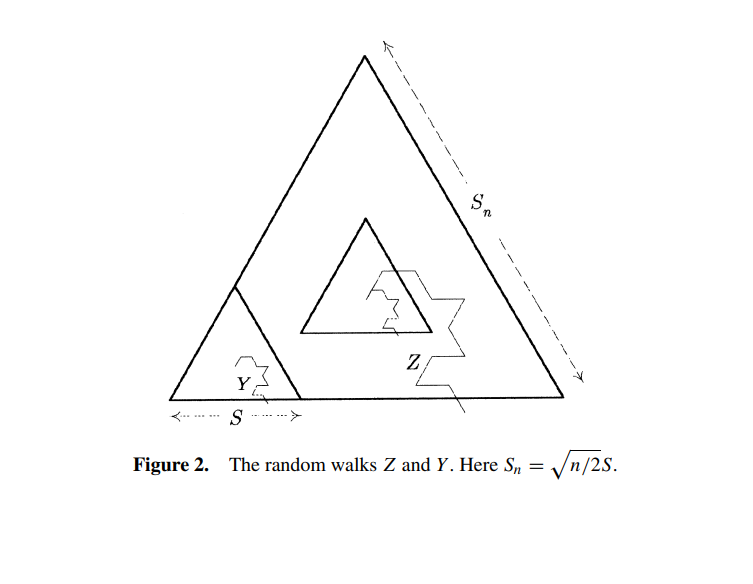
\includegraphics[width=0.4\textwidth]{Screenshot 2025-07-03 132030.png}
    \caption{Exit of Brownian Motion from a Square}
\end{figure}

\begin{proof}
\noindent From the definition of $Z^n$ we have,
\[
Z^n_{T(Z^n, \Delta, \sqrt{n/2}S)} = \sqrt{n/2}(\alpha, \beta) + 
\sum_{i=1}^{\lfloor T(Z^n, \Delta, \sqrt{n/2}S) \rfloor} \xi_i + 
\lambda \xi_{\lfloor T(Z^n, \Delta, \sqrt{n/2}S) \rfloor + 1}
\]
$\lambda \in [0, 1]$. Define $\tilde{Y}^n$ defined as $Y^n$ but starting at $\sqrt{n/2}(\alpha, \beta)$, we can write,
\[
\tilde{Y}^n_{T(Z^n, \Delta, \sqrt{n/2}S)} = \sqrt{n/2}(\alpha, \beta) + \sqrt{2/n} \left( 
\sum_{i=1}^{\lfloor T(Z^n, \Delta, \sqrt{n/2}S) \rfloor} \xi_i + 
\lambda \xi_{\lfloor T(Z^n, \Delta, \sqrt{n/2}S) \rfloor + 1}
\right),
\]
\noindent It is a point in the line segment joining $Z^n_0$ and $Z^n_{T(Z^n, \Delta, \sqrt{n/2}S)}$, whose distance from $Z^n_0$ is $\sqrt{2/n}$ times the length of that segment. Consider the translation of $\Delta_S$ by the vector $(1 - \sqrt{2/n})\sqrt{n/2}(\alpha, \beta)$. Then we get the process  $Y^n$ starting at $(\alpha,\beta)$ which lies on the edge of $\Delta_S$. Thus we obtain,
\[
T(Y^n, \Delta_S) = T(Z^n, \Delta, \sqrt{n/2}S).
\]

Now, by the definition of $X^n$, it is clear that

\[
T(X^n, \Delta_S) = \frac{1}{n} T(Y^n, \Delta_S).
\]

\end{proof}
This lemma will help us to calculate the explicit form of the expected exit time.
\begin{proposition}\cite[Proposition 7]{research}
The limit of the expected exit times from $\triangle_S$ of the approximating random walks $X^n$ is
\[
\frac{ \sqrt{3}\beta \left( \alpha - \frac{1}{\sqrt{3}}\beta \right) \left( S - \alpha - \frac{1}{\sqrt{3}}\beta \right) }{S}, \tag{14}
\]
where $(\alpha, \beta)$ is the starting point.

\end{proposition}
\begin{proof}



The set
\begin{align*}
\big\{(\alpha, \beta) \in \Delta_s :\ 
\sqrt{n/2}(\alpha, \beta)\ 
\text{ is a vertex of the triangular lattice for infinitely many } n\big\}
\end{align*}
is dense in $\Delta_s$.
Define
\[
m =[\sqrt{n/2}S] + 1
\]

For $k = m - 1, m$,
\[
a_k = \frac{\sqrt{n/2} \cdot 2}{\sqrt{3}} \beta
\]
\[
b_k = {\sqrt{n/2}}\left( \alpha - \frac{1}{\sqrt{3}} \beta \right)
\]
\[
c_k = k - \sqrt{n/2} \left( \alpha + \frac{1}{\sqrt{3}} \beta \right)
\]

which follows that
\[
E\left( T(Z^n, \Delta_k) \right) = n \sqrt{3} \beta \left( \alpha - \frac{1}{\sqrt{3}} \beta \right)
= \frac{k - \sqrt{n/2} \alpha - \sqrt{n/2} \left( \frac{1}{\sqrt{3}} \beta \right)}{k}
\]

From the previous lemma,
\[
\frac{1}{n} T\left(Z^n, \Delta_k\right) = T\left(X^n ,\Delta_{k/\sqrt{n/2}} \right)
\]

Thus we have
\[
\Delta_{(m-1)/\sqrt{n/2}} \subseteq \Delta_S \subseteq \Delta_{m/\sqrt{n/2}}
\]
Taking $n \to \infty$
\[
\lim_{n \to \infty} \mathbb{E}[T(X_n, \Delta_{S})] = 
\frac{ \sqrt{3}\beta\left(\alpha - \frac{1}{\sqrt{3}}\beta\right)\left(S - \alpha - \frac{1}{\sqrt{3}}\beta\right) }{S}
\]
\end{proof}
\noindent Thus we get the required explicit form.
\chapter{Further Extensions}
We can cover a flat plane in complete regular manner only using equilateral triangle, square and hexagon. No other regular n-gon can be used in this case as here it is necessary that in regular pattern each point must be surrounded with no of polygons which must be a factor of 360. For equilateral triangle it is 6, for square it is 4 and for hexagon it is 3. Now we are interested in the expected exit time of a 2-d Brownian motion from this n-gons. In the research paper \cite{research} this is done for equilateral triangle. Now further as an extension of our project we will try to do the same for the square. Analogous methods may also be applicable for the case involving a hexagon.
\section{Expected Exit Time of a Brownian motion from a Square}
Firstly we try relate the exit time of a 2-d Brownian motion from a square with that of a random walk in 2 dimension. Consider $S$ is a positive integer and $\square_S$ is placed on the square lattice of unit length in the 2-d plane in such a way that the vertices of $\square_S$ is any of the vertices of the lattice.
\begin{figure}[htbp]
    \centering
    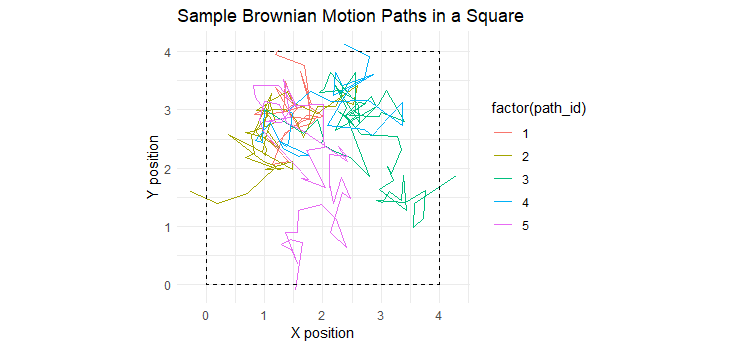
\includegraphics[width=0.8\textwidth]{Exit of BM from Square.png}
    \caption{Exit of Brownian Motion from Square}
\end{figure}
\subsection{2-d Random Walk}
At first let us consider a square of side length $S \in \mathbb{N}$. The vertices of $\square_S$ are $(0,0),(S,0),(0,S),(S,S)$. It is placed on a 2-d plane tiled by square lattice each of unit side length in such a way that the vertices of lattice are the vertices of $\square_S$. Now we simulate this 2-d discrete random walk firstly. Let $h(a,b)$ denote the position of the random walk in 2-d plane. Now starting at any point $(a, b) \in \square_S$ in the next step it has four possible positions to move $(a + 1, b), (a -1, b),(a, b + 1), (a, b - 1)$ each with equal probability.We will stop when $\min\{h(a, b)_1,\, h(a, b)_2,\, S - h(a, b)_1,\, S - h(a, b)_2\} = 0$, where $h(a, b)_i$ denotes the $i$th coordinate of $h(a,b)$. Then the updated number of steps until it stops would be the exit time.

\subsubsection{Code for 2-d Random Walk Generation}
\begin{verbatim}
two_d_rw <- function(S, a, b) {
  count <- 0
  pos <- c(a, b)
  while(min(pos[1], pos[2], S-pos[1], S-pos[2]) != 0) {
    samp <- sample(list(c(1,0), c(0,1), c(-1,0), c(0,-1)), size = 1)
    pos <- pos + samp[[1]]
    count <- count + 1
  }
  return(count)
}    
# Example usage
set.seed(123)
exit_times_discrete <- replicate(1000, two_d_rw(4, 1, 3))
mean_discrete <- mean(exit_times_discrete)
mean_discrete
[1] 2.658
\end{verbatim}

\subsection{The Convergence of the Expected Exit Time}
Define $\xi_i=(cos(k\pi/2),sin(k\pi/2))$ sequence of iid rv where $k=1,2,3,4$. $k$ can take any of the values with equal probability. After this we follow the same arguements which we proved in case of the equilateral triangle and conclude that 
\[
\lim_{n \to \infty} \mathbb{E}\left[T(X_n, \square_S)\right] = \mathbb{E}\left[T(B, \square_S)\right]
\]
notations are followed from Chapter \ref{sec4}. We do the simulation for this.
\subsubsection{Code for 2-d Brownian Motion Generation}
\begin{verbatim}
    simulate_exit_time <- function(S, a, b, dt = 0.01) {
  if (a <= 0 || a >= S || b <= 0 || b >= S) {
    stop("Starting point must be strictly inside the square.")
  }
  
  x <- a
  y <- b
  t <- 0
  
  while (x > 0 && x < S && y > 0 && y < S) {
    x <- x + sqrt(dt) * rnorm(1)
    y <- y + sqrt(dt) * rnorm(1)
    t <- t + dt
  }
  
  return(t)
}
# Example usage
set.seed(123)
exit_times_continuous <- replicate(1000, simulate_exit_time(4, 1, 3))
mean_continuous <- mean(exit_times_continuous)
mean_continuous
[1] 1.61825
\end{verbatim}
\subsubsection{Code for Visualization of Convergence}
\begin{verbatim}
library(ggplot2)
# Create data frames
df_discrete <- data.frame(Time = exit_times_discrete, Type = "Discrete")
df_continuous <- data.frame(Time = exit_times_continuous, Type = "Continuous")
df_combined <- rbind(df_discrete, df_continuous)
# Plot histograms
ggplot(df_combined, aes(x = Time, fill = Type)) +
  geom_histogram(alpha = 0.6, position = "identity", bins = 30) +
  facet_wrap(~Type, scales = "free") +
  labs(title = "Exit Time Distributions",
       x = "Exit Time",
       y = "Frequency") +
  theme_minimal()
\end{verbatim}

\subsubsection{Visualization of Convergence in Distribution}
In the picture below we can see that both of them have the same distributional structure which implies the convergence in distribution.

\vspace{1 cm}
\begin{figure}[htbp]
    \centering
    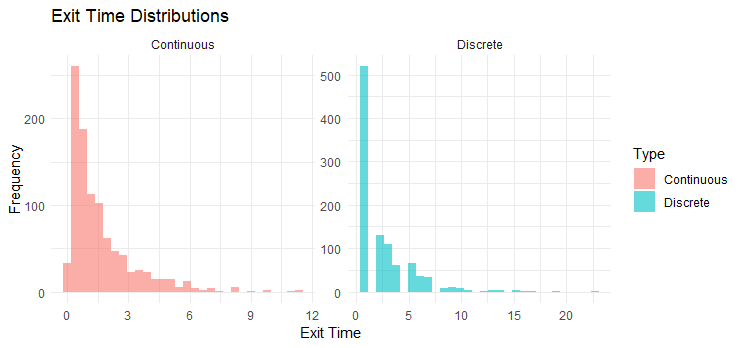
\includegraphics[width=0.8\textwidth]{Distribution Convergence.png}
    \caption{Convergence in Distribution}
\end{figure}
\section{Closed form Expression of the Expected Exit Time}
Now our main aim is to get a closed form expression for the expected exit time of Brownian motion starting at $(a,b) \in \square_S$ from a square of side length $S$. Define $k(a,b)$ as the expected exit time. Then we are to solve the difference equation 
\[
k(a,b)=1+(1/4)(k(a+1,b)+k(a-1,b)+k(a,b+1)+k(a,b-1))
\]
with boundary conditions
\[
k(a,b)=0 \text{ when min\{a,b,S-a,S-b\}=0}
\]
\chapter{Conclusion}
Owing to the limited time available within the scope of this project, I was unable to derive a complete closed-form solution. However, the progress made lays a strong foundation, and I intend to continue this work beyond the current timeline to explore the problem further and aim for a complete analytical resolution.


% -------------------------
% Bibliography
% -------------------------
\bibliographystyle{plain}
\bibliography{references}

\end{document}
